\documentclass[border=5mm]{standalone}
\usepackage{tikz}
\usepackage{tikz-qtree}

\begin{document}
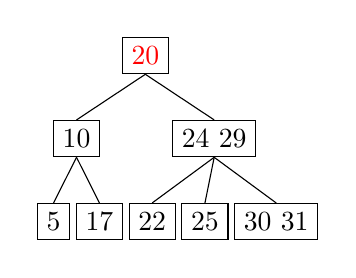
\begin{tikzpicture}[every tree node/.style={align=center}]
    \matrix[row sep=1cm, column sep=1cm] {
    \Tree
    [.\node[draw, rectangle]{\textcolor{red}{20}};
    [.\node[draw, rectangle]{10};
    [.\node[draw, rectangle]{5}; ]
    [.\node[draw, rectangle]{17};  ]
    ]
    [.\node[draw, rectangle]{24 29};
    [.\node[draw, rectangle]{22};    ]
    [.\node[draw, rectangle]{25};    ]
    [.\node[draw, rectangle]{30 31};    ]
    ]
    ]; \\
    };
\end{tikzpicture}
\end{document}